\subsection{Bestimmung der Brechungsindices}

Zur Messung des Brechnungsindex benutzen wir einen Prismenspektralapparat.
Dabei ist ein Glasprisma auf dem Drehteil eines Goniometers montiert. Durch
einen Spalt und eine Sammellinse fällt Licht aus einer Heliumlampe auf
das Prisma. Dadurch, dass der Spalt in der Brennebene der Linse steht, erhalten
wir paralleles Licht. Nach der Brechung fällt das Licht in die Brennebene einer Lupe, durch welche wir
die Spektrallinien sehen können.
Da wir nur den symmetrischen Fall betrachten, bei dem a = a' und b = b'
ist, folgt
\begin{align}
n=\frac{sin(\frac{\varphi + \eta}{2})}{sin(\frac{\varphi}{2})}\nonumber
\end{align}

Um sicherzustellen, dass ein symmertrischer Strahlenverlauf vorliegt, bringt
man den gebrochenen Strahl mit dem an der Basis des Prismas reflektrierten
Strahl zur Deckung. Dann misst man die Auslenkung des gebrochenen Strahles
links und rechts und berechnet den Brechnungswinkel wie folgt:

\begin{align}
-\eta=180^\circ +\Omega_l - \Omega_r \nonumber
\end{align}

Weiterhin sollte der Winkel an der brechenden Kante gemessen. Dafür wurde
diese Kante auf das Kollimatorrohr gerichtet und der Winkel des reflektierten
Strahles gemessen. Dieser Winkel wurde auf beiden Seiten fünf mal abgelesen,
wobei das Prisma mit der brechenden Kante über den Strahl hinweg auf eine
spiegelverkehrte Position gedreht wurde. Damit ergibt sich mit der Formel:

\begin{align}
\varphi=180^\circ +\varphi_l - \varphi_r \nonumber
\end{align}

\begin{table}[h]
\begin{center}
\begin{tabular}[c]{|c|c|c|} \hline
$\varphi_l$ in $^\circ$ & $\varphi_r$ in $^\circ$ & $\varphi$  in $^\circ$\\ \hline
263,9 & 23,6+360 & 60,3 \\ 
229,2 & 349,2 & 60 \\ 
229,5 & 349,3 & 60,2 \\ 
241,4 & 1,5+360 & 60,1 \\ 
240,0 & 360,0 & 60,3 \\ \hline
\end{tabular}
\caption{Winkel $\Phi$ an der brechenden Kante des Prismas}
\end{center}
\end{table}
% \newpage

Somit lautet der Mittelwert:
$\varphi = 60, 18^\circ \pm 0, 58^\circ$ Der Fehler wird mit der Formel der Standardabweichung des Mittelwertes
berechnet.

Für die Indicies n und $\eta$ folgt damit:
\begin{table}[h]
\begin{center}
\begin{tabular}[c]{|c|c|c|c|c|c|} \hline
Farbe & $\lambda$ in nm & $\Omega_l$  in $^\circ$ & $\Omega_r$  in $^\circ$ & $\eta$  in $^\circ$ & n \\ \hline
Rot & 632,8 & 147,5 & 27,5 +360 & 60 & 1,729\\
Gelb & 594,1 & 147,3 & 27,2+360 & 59,9 & 1,728\\
Gr"un & 543,5 & 146,8 & 26,7+360 & 59,9 & 1,728\\
Blau & kA & 146,4 & 26,2+360 &  59,8 & 1,727\\ \hline
\end{tabular}
\caption{Brechungsindicies n und $\eta$}
\end{center}
\end{table}

\subsection{Bestimmung der Dispersionskurve}

Um die Dispersionskurve zu bestimmen, werden die Quadrate der Brechungsindize
gegen Quadrate der Wellenlängen und einmal gegen die Kehrwerte der Wellenlängenquadrate.
Somit kann man mit einer linearen Regression y = mx + b bestimmen, durch die Abweichung der
Kurve von den Messwerten kann bestimmt werden, welche Dispersionskurve die richtige ist.
Aus der Ausgleichsrechnung ergibt sich für $n^2$ gegen $\lambda^{-2}$ 
 \begin{align}
n^2( \lambda ) = (-0,302 \pm 0,241) \mu m^{2} \lambda^{-2} + 2,996 \pm 0,007\nonumber
\end{align}
und für $n^2$ gegen $\lambda^2$ ergibt sich
\begin{align}
n'^2( \lambda ) = (0,273 \pm 0,183) \mu m^{-2} \lambda^2 + 2,977 \pm 0,006 \nonumber
\end{align}

Durch die berechnung der Abstandsquadrate $s_n$ und $s_n'$ folgt die richtige Dispersionskurve.
 \begin{align}
s_n=2,3043\nonumber
\end{align}
\begin{align}
s_n'=0,0193\nonumber
\end{align}
Woraus folgt, dass die Dispersionskurve die gültige ist und folgendermaßen aussieht:

\begin{figure}[h]
	\centering
		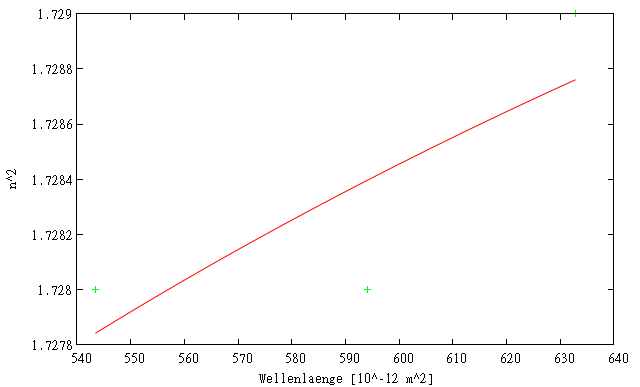
\includegraphics[width=1.00\textwidth]{Plot1B.png}
		\caption{Dispersionskurve}
	\label{fig:Plot}
\end{figure}

\subsection{Bestimmung der Abbesche Zahl}
Zur Berechung der Abbeschen Zahl benötigt man die Formel
\begin{align}
v=\frac{n_D-1}{n_F-n_C}\nonumber
\end{align}
Für die man die Brechungsindizes der FRAUNHOFER'schen Linien benötigt. Diese erhält man
indem man $\lambda_C$= 656nm,$\lambda_D$ = 589nm und $\lambda_F$ = 486nm in die Formel einsetzt.
Dabei muss man beachten, dass $A_0$ und $A_2$ fehlerbehaftet sind, da die Messergebnisse,wie in der Diskussion
erläutert große Fehler aufweisen wird auf die Fehlerfortpflanzung an dieser Stelle verzichtet.

Somit folgt:

\begin{align}
n_C= 2,294\nonumber
\end{align}
\begin{align}
n_D= 2,125\nonumber
\end{align}
\begin{align}
n_F= 1,717\nonumber
\end{align}
\begin{align}
v= -1,950 \nonumber
\end{align}




